\documentclass{beamer}
\let\vec\mathbf
\mode<presentation>
\usepackage{amsmath}
\usepackage{amssymb}
%\usepackage{advdate}
\usepackage{adjustbox}
%\usepackage{subcaption}
\usepackage{enumitem}
\usepackage{multicol}
\usepackage{mathtools}
\usepackage{listings}
\usepackage{url}
\usetheme{Boadilla}
\usecolortheme{lily}
\setbeamertemplate{footline}
{
  \leavevmode%
  \hbox{%
  \begin{beamercolorbox}[wd=\paperwidth,ht=2.25ex,dp=1ex,right]{author in head/foot}%
    \insertframenumber{} / \inserttotalframenumber\hspace*{2ex} 
  \end{beamercolorbox}}%
  \vskip0pt%
}
\setbeamertemplate{navigation symbols}{}
\providecommand{\nCr}[2]{\,^{#1}C_{#2}} % nCr
\providecommand{\nPr}[2]{\,^{#1}P_{#2}} % nPr
\providecommand{\mbf}{\mathbf}
\providecommand{\pr}[1]{\ensuremath{\Pr\left(#1\right)}}
\providecommand{\qfunc}[1]{\ensuremath{Q\left(#1\right)}}
\providecommand{\sbrak}[1]{\ensuremath{{}\left[#1\right]}}
\providecommand{\lsbrak}[1]{\ensuremath{{}\left[#1\right.}}
\providecommand{\rsbrak}[1]{\ensuremath{{}\left.#1\right]}}
\providecommand{\brak}[1]{\ensuremath{\left(#1\right)}}
\providecommand{\lbrak}[1]{\ensuremath{\left(#1\right.}}
\providecommand{\rbrak}[1]{\ensuremath{\left.#1\right)}}
\providecommand{\cbrak}[1]{\ensuremath{\left\{#1\right\}}}
\providecommand{\lcbrak}[1]{\ensuremath{\left\{#1\right.}}
\providecommand{\rcbrak}[1]{\ensuremath{\left.#1\right\}}}
\theoremstyle{remark}
\newtheorem{rem}{Remark}
\newcommand{\sgn}{\mathop{\mathrm{sgn}}}

\providecommand{\res}[1]{\Res\displaylimits_{#1}} 
\providecommand{\norm}[1]{\lVert#1\rVert}
\providecommand{\mtx}[1]{\mathbf{#1}}

\providecommand{\fourier}{\overset{\mathcal{F}}{ \rightleftharpoons}}
%\providecommand{\hilbert}{\overset{\mathcal{H}}{ \rightleftharpoons}}
\providecommand{\system}{\overset{\mathcal{H}}{ \longleftrightarrow}}
	%\newcommand{\solution}[2]{\textbf{Solution:}{#1}}
%\newcommand{\solution}{\noindent \textbf{Solution: }}
\providecommand{\dec}[2]{\ensuremath{\overset{#1}{\underset{#2}{\gtrless}}}}
\newcommand{\myvec}[1]{\ensuremath{\begin{pmatrix}#1\end{pmatrix}}}

\title{Matrices in Geometry - 2.10.64}
\author{EE25BTECH11035  Kushal B N}
\date{Sep, 2025}

\begin{document}

\maketitle

\section{Problem Statement}
\begin{frame}
\frametitle{Problem Statement}
The position vectors of the points $\vec{A}$, $\vec{B}$, $\vec{C}$ and $\vec{D}$ are $\brak{3\hat{i}-2\hat{j}-\hat{k}}$, $\brak{2\hat{i}+3\hat{j}-4\hat{k}}$, $\brak{-\hat{i}+\hat{j}+2\hat{k}}$ and $\brak{4\hat{i}+5\hat{j}+\lambda\hat{k}}$ respectively. If the points $\vec{A}$, $\vec{B}$, $\vec{C}$ and $\vec{D}$ lie on a plane, find the value of $\lambda$.

\end{frame}

\section{Solution}
\begin{frame}{Solution}
Given,\\
$\vec{A}\myvec{3\\-2\\-1}$, $\vec{B}\myvec{2\\3\\-4}$, $\vec{C}\myvec{-1\\1\\2}$ and $\vec{D}\myvec{4\\5\\\lambda}$.

The general equation for a plane with normal vector $\vec{n}$ passing through point P is \\
\begin{equation}
    \vec{n}^{\top}\vec{P} = d
\end{equation}
So,
\begin{equation}
    \vec{n}^{\top}\vec{A} = d
\end{equation}

\begin{equation}
    \vec{n}^{\top}\vec{B} = d
\end{equation}

\begin{equation}
    \vec{n}^{\top}\vec{C} = d
\end{equation}

\begin{equation}
    \vec{n}^{\top}\vec{D} = d
\end{equation}

\end{frame}

\begin{frame}{Solution}
Forming direction vectors in the plane,

\begin{equation}
\vec{B} - \vec{A} = \myvec{-1\\5\\-3}
\end{equation}

\begin{equation}
\vec{C} - \vec{A} = \myvec{-4\\3\\3}
\end{equation}

Now, the normal vector will be orthogonal to both of these direction vectors, so that
\begin{equation}
    \brak{\vec{B} - \vec{A}}^{\top}\vec{n} = 0
\end{equation}

\begin{equation}
    \brak{\vec{C} - \vec{A}}^{\top}\vec{n} = 0
\end{equation}

\end{frame}

\begin{frame}{Solution}
Combining the above two equations,
\begin{equation}
    \myvec{\brak{\vec{B} - \vec{A}}^{\top}\\ \brak{\vec{C} - \vec{A}}^{\top}}\vec{n} = 0
\end{equation}

\begin{equation}
    \myvec{-1&5&-3\\-4&3&3}\vec{n} = \myvec{0\\0}
\end{equation}

Augmented matrix:
\begin{equation}
    \implies \myvec{-1&5&-3&|&0\\-4&3&3&|&0}
\end{equation}

\begin{equation}
    \myvec{-1&5&-3&|&0\\-4&3&3&|&0} \overset{R_2 \rightarrow R_2 - 4R_1}{\longrightarrow} \myvec{-1&5&-3&|&0\\0&-17&15&|&0}
\end{equation}
\end{frame}

\begin{frame}{Solution}
\begin{equation}
    \myvec{-1&5&-3&|&0\\0&-17&15&|&0} \overset{R_2 \rightarrow \frac{-1}{17}R_2}{\longrightarrow} \myvec{-1&5&-3&|&0\\0&1&\frac{-15}{17}&|&0}
\end{equation}

\begin{equation}
    \myvec{-1&5&-3&|&0\\0&1&\frac{-15}{17}&|&0} \overset{R_1 \rightarrow R_1 - 5R_2}{\longrightarrow} \myvec{-1&0&\frac{24}{17}&|&0\\0&1&\frac{-15}{17}&|&0}
\end{equation}

\begin{equation}
    \implies \vec{n} = \myvec{\frac{24}{17}\\ \frac{15}{17}\\ 1} t
\end{equation}

So we can take $t=17$ in order to get integer coefficients,
\begin{equation}
    \vec{n} = \myvec{24\\15\\17}
\end{equation}

\end{frame}

\begin{frame}{Solution}
Substituting this in (2),
\begin{equation}
    d = \myvec{24&15&17}\myvec{3\\-2\\-1} = 25
\end{equation}

So substituting for $\vec{D}$ and $d$ in the equation (5), we have
\begin{equation}
    \myvec{24&15&17}\myvec{4\\5\\\lambda} = 25
\end{equation}

\begin{equation}
    \implies \fbox{$\lambda = \frac{-146}{17}$}
\end{equation}
\end{frame}
\section{Final Answer}
\begin{frame}{Final Answer}
The value of $\lambda$ is $\frac{-146}{17}$.

\begin{figure}
    \centering
    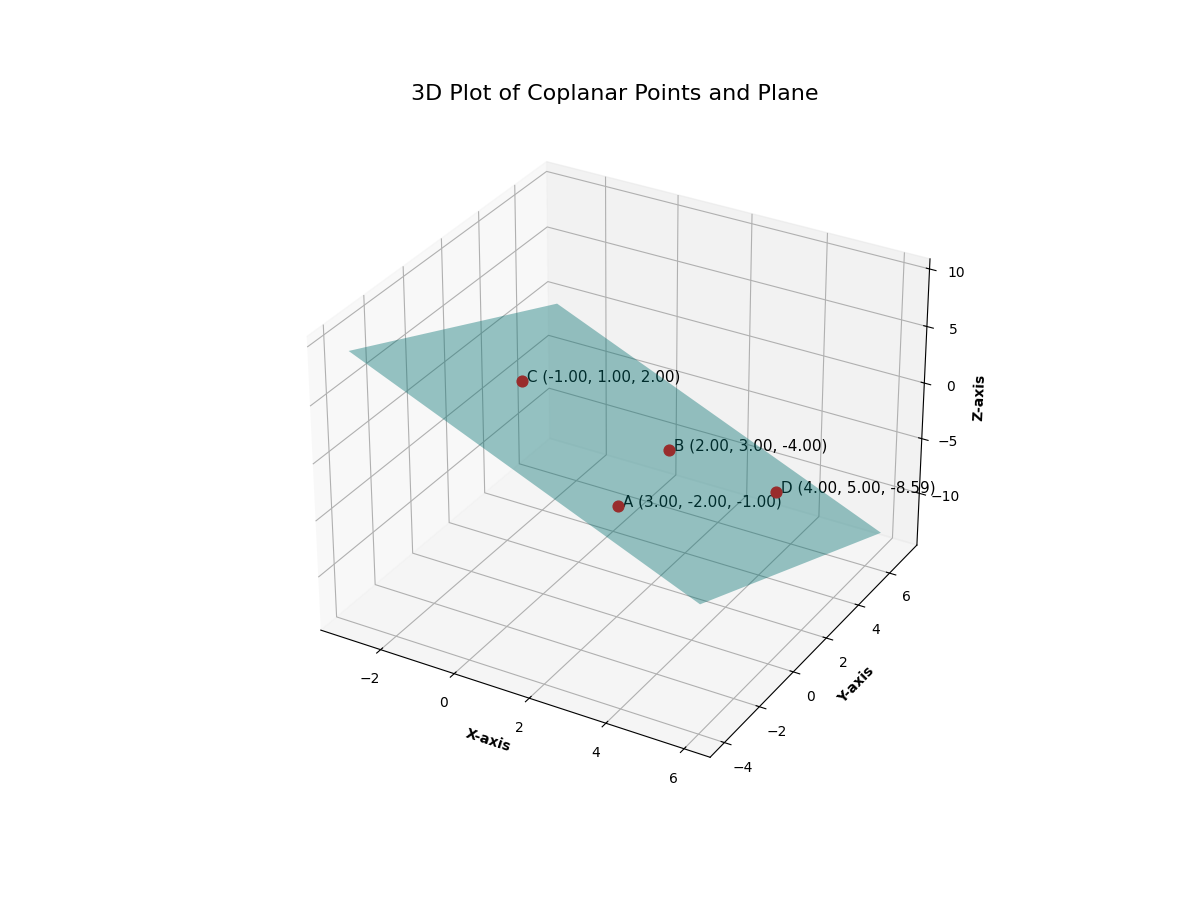
\includegraphics[width=0.95\columnwidth]{figs/2.png}
\end{figure}
\end{frame}
\end{document}